\chapter{Vahvasti yhtenäisyys}

\index{vahvasti yhtenäinen verkko}

Suunnatussa verkossa yhtenäisyys ei takaa sitä,
että kahden solmun välillä olisi olemassa polkua,
koska kaarten suunnat rajoittavat liikkumista.
Niinpä suunnattuja verkkoja varten on mielekästä
määritellä uusi käsite,
joka vaatii enemmän verkon yhtenäisyydeltä.

Verkko on \key{vahvasti yhtenäinen},
jos mistä tahansa solmusta on olemassa polku
kaikkiin muihin solmuihin.
Esimerkiksi seuraavassa kuvassa vasen
verkko on vahvasti yhtenäinen,
kun taas oikea verkko ei ole.

\begin{center}
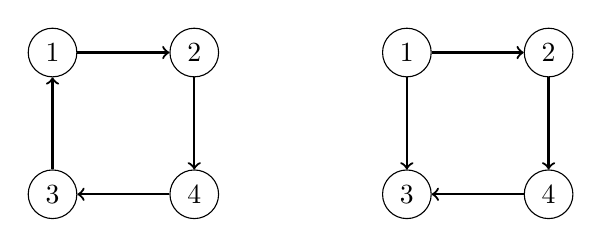
\begin{tikzpicture}[scale=0.9]
\node[draw, circle] (1) at (1,1) {$1$};
\node[draw, circle] (2) at (3,1) {$2$};
\node[draw, circle] (3) at (1,-1) {$3$};
\node[draw, circle] (4) at (3,-1) {$4$};

\path[draw,thick,->] (1) -- (2);
\path[draw,thick,->] (2) -- (4);
\path[draw,thick,->] (4) -- (3);
\path[draw,thick,->] (3) -- (1);

\node[draw, circle] (1b) at (6,1) {$1$};
\node[draw, circle] (2b) at (8,1) {$2$};
\node[draw, circle] (3b) at (6,-1) {$3$};
\node[draw, circle] (4b) at (8,-1) {$4$};

\path[draw,thick,->] (1b) -- (2b);
\path[draw,thick,->] (2b) -- (4b);
\path[draw,thick,->] (4b) -- (3b);
\path[draw,thick,->] (1b) -- (3b);
\end{tikzpicture}
\end{center}

Oikeanpuoleinen verkko ei ole vahvasti yhtenäinen,
koska esimerkiksi solmusta 2 ei ole
polkua solmuun 1.

\index{vahvasti yhtenäinen komponentti}
\index{komponenttiverkko}

Verkon \key{vahvasti yhtenäiset komponentit}
jakavat verkon solmut mahdollisimman
suuriin vahvasti yhtenäisiin osiin.
Verkon vahvasti yhtenäiset komponentit
muodostavat syklittömän \key{komponenttiverkon},
joka kuvaa alkuperäisen verkon syvärakennetta.

Esimerkiksi verkon

\begin{center}
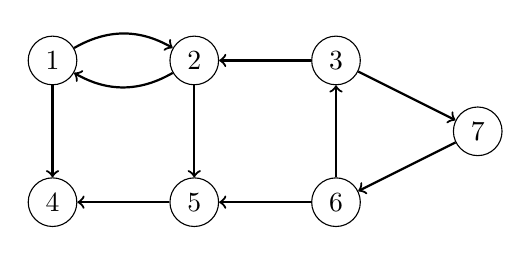
\begin{tikzpicture}[scale=0.9,label distance=-2mm]
\node[draw, circle] (1) at (-1,1) {$7$};
\node[draw, circle] (2) at (-3,2) {$3$};
\node[draw, circle] (4) at (-5,2) {$2$};
\node[draw, circle] (6) at (-7,2) {$1$};
\node[draw, circle] (3) at (-3,0) {$6$};
\node[draw, circle] (5) at (-5,0) {$5$};
\node[draw, circle] (7) at (-7,0) {$4$};

\path[draw,thick,->] (2) -- (1);
\path[draw,thick,->] (1) -- (3);
\path[draw,thick,->] (3) -- (2);
\path[draw,thick,->] (2) -- (4);
\path[draw,thick,->] (3) -- (5);
\path[draw,thick,->] (4) edge [bend left] (6);
\path[draw,thick,->] (6) edge [bend left] (4);
\path[draw,thick,->] (4) -- (5);
\path[draw,thick,->] (5) -- (7);
\path[draw,thick,->] (6) -- (7);
\end{tikzpicture}
\end{center}

vahvasti yhtenäiset komponentit ovat

\begin{center}
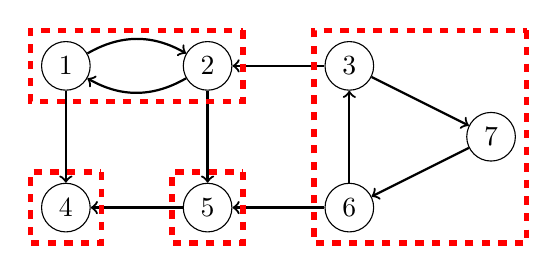
\begin{tikzpicture}[scale=0.9]
\node[draw, circle] (1) at (-1,1) {$7$};
\node[draw, circle] (2) at (-3,2) {$3$};
\node[draw, circle] (4) at (-5,2) {$2$};
\node[draw, circle] (6) at (-7,2) {$1$};
\node[draw, circle] (3) at (-3,0) {$6$};
\node[draw, circle] (5) at (-5,0) {$5$};
\node[draw, circle] (7) at (-7,0) {$4$};

\path[draw,thick,->] (2) -- (1);
\path[draw,thick,->] (1) -- (3);
\path[draw,thick,->] (3) -- (2);
\path[draw,thick,->] (2) -- (4);
\path[draw,thick,->] (3) -- (5);
\path[draw,thick,->] (4) edge [bend left] (6);
\path[draw,thick,->] (6) edge [bend left] (4);
\path[draw,thick,->] (4) -- (5);
\path[draw,thick,->] (5) -- (7);
\path[draw,thick,->] (6) -- (7);

\draw [red,thick,dashed,line width=2pt] (-0.5,2.5) rectangle (-3.5,-0.5);
\draw [red,thick,dashed,line width=2pt] (-4.5,2.5) rectangle (-7.5,1.5);
\draw [red,thick,dashed,line width=2pt] (-4.5,0.5) rectangle (-5.5,-0.5);
\draw [red,thick,dashed,line width=2pt] (-6.5,0.5) rectangle (-7.5,-0.5);
\end{tikzpicture}
\end{center}

ja ne muodostavat seuraavan komponenttiverkon:

\begin{center}
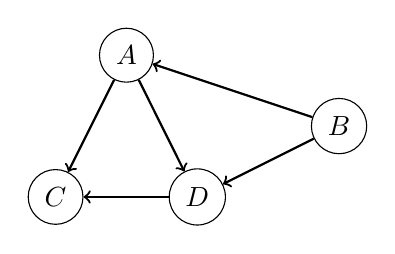
\begin{tikzpicture}[scale=0.9]
\node[draw, circle] (1) at (-3,1) {$B$};
\node[draw, circle] (2) at (-6,2) {$A$};
\node[draw, circle] (3) at (-5,0) {$D$};
\node[draw, circle] (4) at (-7,0) {$C$};

\path[draw,thick,->] (1) -- (2);
\path[draw,thick,->] (1) -- (3);
\path[draw,thick,->] (2) -- (3);
\path[draw,thick,->] (2) -- (4);
\path[draw,thick,->] (3) -- (4);
\end{tikzpicture}
\end{center}

Komponentit ovat $A=\{1,2\}$,
$B=\{3,6,7\}$, $C=\{4\}$ sekä $D=\{5\}$.

Komponenttiverkko on syklitön suunnattu verkko,
jonka käsittely on alkuperäistä verkkoa
helpompaa, koska siinä ei ole syklejä.
Niinpä komponenttiverkolle voi muodostaa
luvun 16 tapaan topologisen järjestyksen
ja soveltaa sen jälkeen dynaamista ohjelmintia
verkon käsittelyyn.

Tutustumme seuraavaksi algoritmiin,
jonka avulla voi etsiä tehokkaasti verkon
vahvasti yhtenäiset komponentit.
Tämän jälkeen näemme, kuinka algoritmia voi
käyttää logiikan 2SAT-ongelman ratkaisemiseen.

\section{Kosarajun algoritmi}

\index{Kosarajun algoritmi}

\key{Kosarajun algoritmi} on tehokas
menetelmä verkon
vahvasti yhtenäisten komponenttien etsimiseen.
Se suorittaa verkkoon
kaksi syvyyshakua, joista ensimmäinen
kerää solmut listaan verkon rakenteen perusteella
ja toinen muodostaa vahvasti yhtenäiset komponentit.

\subsubsection{Syvyyshaku 1}

Algoritmin ensimmäinen vaihe muodostaa listan solmuista
syvyyshaun käsittelyjärjestyksessä.
Algoritmi käy solmut läpi yksi kerrallaan,
ja jos solmua ei ole vielä käsitelty, algoritmi suorittaa
solmusta alkaen syvyyshaun.
Solmu lisätään listalle, kun syvyyshaku on 
käsitellyt kaikki siitä lähtevät kaaret.

Esimerkkiverkossa solmujen käsittelyjärjestys on:
\begin{center}
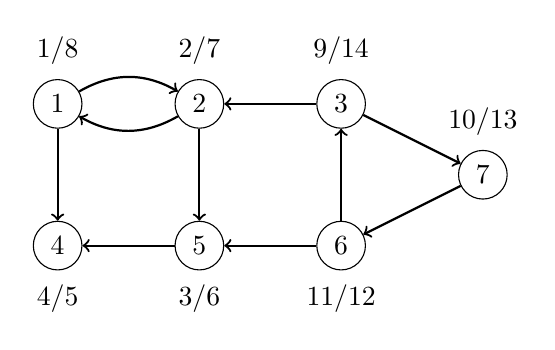
\begin{tikzpicture}[scale=0.9,label distance=-2mm]
\node[draw, circle] (1) at (-1,1) {$7$};
\node[draw, circle] (2) at (-3,2) {$3$};
\node[draw, circle] (4) at (-5,2) {$2$};
\node[draw, circle] (6) at (-7,2) {$1$};
\node[draw, circle] (3) at (-3,0) {$6$};
\node[draw, circle] (5) at (-5,0) {$5$};
\node[draw, circle] (7) at (-7,0) {$4$};

\node at (-7,2.75) {$1/8$};
\node at (-5,2.75) {$2/7$};
\node at (-3,2.75) {$9/14$};
\node at (-7,-0.75) {$4/5$};
\node at (-5,-0.75) {$3/6$};
\node at (-3,-0.75) {$11/12$};
\node at (-1,1.75) {$10/13$};

\path[draw,thick,->] (2) -- (1);
\path[draw,thick,->] (1) -- (3);
\path[draw,thick,->] (3) -- (2);
\path[draw,thick,->] (2) -- (4);
\path[draw,thick,->] (3) -- (5);
\path[draw,thick,->] (4) edge [bend left] (6);
\path[draw,thick,->] (6) edge [bend left] (4);
\path[draw,thick,->] (4) -- (5);
\path[draw,thick,->] (5) -- (7);
\path[draw,thick,->] (6) -- (7);
\end{tikzpicture}
\end{center}

Solmun kohdalla oleva merkintä $x/y$ tarkoittaa, että solmun
käsittely syvyyshaussa alkoi hetkellä $x$ ja päättyi hetkellä $y$.
Kun solmut järjestetään käsittelyn päättymisajan
mukaan, tuloksena on seuraava järjestys:

\begin{tabular}{ll}
\\
solmu & päättymisaika \\
\hline
4 & 5 \\
5 & 6 \\
2 & 7 \\
1 & 8 \\
6 & 12 \\
7 & 13 \\
3 & 14 \\
\\
\end{tabular}

Solmujen käsittelyjärjestys algoritmin seuraavassa vaiheessa
tulee olemaan tämä järjestys käänteisenä eli $[3,7,6,1,2,5,4]$.

\subsubsection{Syvyyshaku 2}

Algoritmin toinen vaihe muodostaa verkon vahvasti
yhtenäiset komponentit.
Ennen toista syvyyshakua algoritmi muuttaa
jokaisen kaaren suunnan käänteiseksi.
Tämä varmistaa,
että toisen syvyyshaun aikana löydetään
joka kerta vahvasti yhtenäinen komponentti,
johon ei kuulu ylimääräisiä solmuja.

Esimerkkiverkko on käännettynä seuraava:

\begin{center}
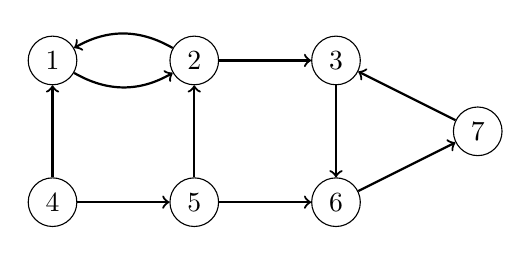
\begin{tikzpicture}[scale=0.9,label distance=-2mm]
\node[draw, circle] (1) at (-1,1) {$7$};
\node[draw, circle] (2) at (-3,2) {$3$};
\node[draw, circle] (4) at (-5,2) {$2$};
\node[draw, circle] (6) at (-7,2) {$1$};
\node[draw, circle] (3) at (-3,0) {$6$};
\node[draw, circle] (5) at (-5,0) {$5$};
\node[draw, circle] (7) at (-7,0) {$4$};

\path[draw,thick,<-] (2) -- (1);
\path[draw,thick,<-] (1) -- (3);
\path[draw,thick,<-] (3) -- (2);
\path[draw,thick,<-] (2) -- (4);
\path[draw,thick,<-] (3) -- (5);
\path[draw,thick,<-] (4) edge [bend left] (6);
\path[draw,thick,<-] (6) edge [bend left] (4);
\path[draw,thick,<-] (4) -- (5);
\path[draw,thick,<-] (5) -- (7);
\path[draw,thick,<-] (6) -- (7);
\end{tikzpicture}
\end{center}

Tämän jälkeen algoritmi käy läpi
solmut käänteisessä ensimmäisen syvyyshaun
tuottamassa järjestyksessä.
Jos solmu ei kuulu vielä komponenttiin,
siitä alkaa uusi syvyyshaku.
Solmun komponenttiin liitetään kaikki aiemmin
käsittelemättömät solmut,
joihin syvyyshaku pääsee solmusta.

Esimerkkiverkossa muodostuu ensin komponentti
solmusta 3 alkaen:

\begin{center}
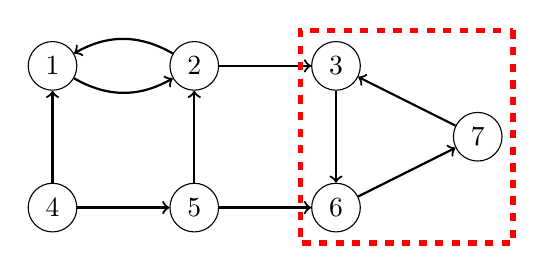
\begin{tikzpicture}[scale=0.9,label distance=-2mm]
\node[draw, circle] (1) at (-1,1) {$7$};
\node[draw, circle] (2) at (-3,2) {$3$};
\node[draw, circle] (4) at (-5,2) {$2$};
\node[draw, circle] (6) at (-7,2) {$1$};
\node[draw, circle] (3) at (-3,0) {$6$};
\node[draw, circle] (5) at (-5,0) {$5$};
\node[draw, circle] (7) at (-7,0) {$4$};

\path[draw,thick,<-] (2) -- (1);
\path[draw,thick,<-] (1) -- (3);
\path[draw,thick,<-] (3) -- (2);
\path[draw,thick,<-] (2) -- (4);
\path[draw,thick,<-] (3) -- (5);
\path[draw,thick,<-] (4) edge [bend left] (6);
\path[draw,thick,<-] (6) edge [bend left] (4);
\path[draw,thick,<-] (4) -- (5);
\path[draw,thick,<-] (5) -- (7);
\path[draw,thick,<-] (6) -- (7);

\draw [red,thick,dashed,line width=2pt] (-0.5,2.5) rectangle (-3.5,-0.5);
%\draw [red,thick,dashed,line width=2pt] (-4.5,2.5) rectangle (-7.5,1.5);
%\draw [red,thick,dashed,line width=2pt] (-4.5,0.5) rectangle (-5.5,-0.5);
%\draw [red,thick,dashed,line width=2pt] (-6.5,0.5) rectangle (-7.5,-0.5);
\end{tikzpicture}
\end{center}

Huomaa, että kaarten kääntämisen ansiosta komponentti
ei pääse ''vuotamaan'' muihin verkon osiin.

\begin{samepage}
Sitten listalla ovat solmut 7 ja 6, mutta ne on jo liitetty
komponenttiin.
Seuraava uusi solmu on 1, josta muodostuu uusi komponentti:

\begin{center}
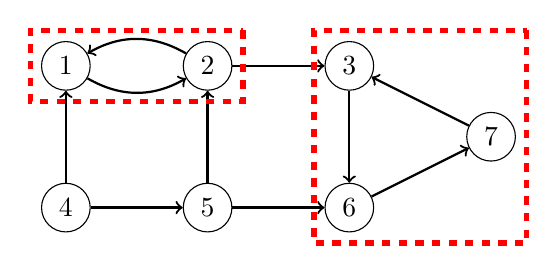
\begin{tikzpicture}[scale=0.9,label distance=-2mm]
\node[draw, circle] (1) at (-1,1) {$7$};
\node[draw, circle] (2) at (-3,2) {$3$};
\node[draw, circle] (4) at (-5,2) {$2$};
\node[draw, circle] (6) at (-7,2) {$1$};
\node[draw, circle] (3) at (-3,0) {$6$};
\node[draw, circle] (5) at (-5,0) {$5$};
\node[draw, circle] (7) at (-7,0) {$4$};

\path[draw,thick,<-] (2) -- (1);
\path[draw,thick,<-] (1) -- (3);
\path[draw,thick,<-] (3) -- (2);
\path[draw,thick,<-] (2) -- (4);
\path[draw,thick,<-] (3) -- (5);
\path[draw,thick,<-] (4) edge [bend left] (6);
\path[draw,thick,<-] (6) edge [bend left] (4);
\path[draw,thick,<-] (4) -- (5);
\path[draw,thick,<-] (5) -- (7);
\path[draw,thick,<-] (6) -- (7);

\draw [red,thick,dashed,line width=2pt] (-0.5,2.5) rectangle (-3.5,-0.5);
\draw [red,thick,dashed,line width=2pt] (-4.5,2.5) rectangle (-7.5,1.5);
%\draw [red,thick,dashed,line width=2pt] (-4.5,0.5) rectangle (-5.5,-0.5);
%\draw [red,thick,dashed,line width=2pt] (-6.5,0.5) rectangle (-7.5,-0.5);
\end{tikzpicture}
\end{center}
\end{samepage}

Viimeisenä algoritmi käsittelee solmut 5 ja 4,
jotka tuottavat loput vahvasti yhtenäiset komponentit:

\begin{center}
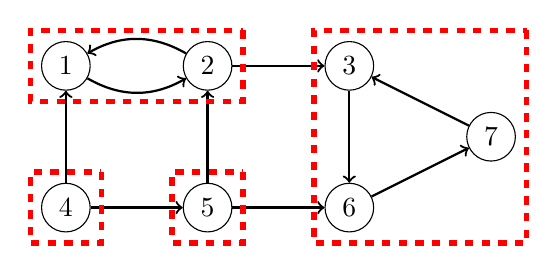
\begin{tikzpicture}[scale=0.9,label distance=-2mm]
\node[draw, circle] (1) at (-1,1) {$7$};
\node[draw, circle] (2) at (-3,2) {$3$};
\node[draw, circle] (4) at (-5,2) {$2$};
\node[draw, circle] (6) at (-7,2) {$1$};
\node[draw, circle] (3) at (-3,0) {$6$};
\node[draw, circle] (5) at (-5,0) {$5$};
\node[draw, circle] (7) at (-7,0) {$4$};

\path[draw,thick,<-] (2) -- (1);
\path[draw,thick,<-] (1) -- (3);
\path[draw,thick,<-] (3) -- (2);
\path[draw,thick,<-] (2) -- (4);
\path[draw,thick,<-] (3) -- (5);
\path[draw,thick,<-] (4) edge [bend left] (6);
\path[draw,thick,<-] (6) edge [bend left] (4);
\path[draw,thick,<-] (4) -- (5);
\path[draw,thick,<-] (5) -- (7);
\path[draw,thick,<-] (6) -- (7);

\draw [red,thick,dashed,line width=2pt] (-0.5,2.5) rectangle (-3.5,-0.5);
\draw [red,thick,dashed,line width=2pt] (-4.5,2.5) rectangle (-7.5,1.5);
\draw [red,thick,dashed,line width=2pt] (-4.5,0.5) rectangle (-5.5,-0.5);
\draw [red,thick,dashed,line width=2pt] (-6.5,0.5) rectangle (-7.5,-0.5);
\end{tikzpicture}
\end{center}

Algoritmin aikavaativuus on $O(n+m)$,
missä $n$ on solmujen määrä ja $m$ on kaarten määrä.
Tämä johtuu siitä,
että algoritmi suorittaa kaksi syvyyshakua ja
kummankin haun aikavaativuus on $O(n+m)$.

\section{2SAT-ongelma}

\index{2SAT-ongelma}

Vahvasti yhtenäisyys liittyy myös \key{2SAT-ongelman} ratkaisemiseen.
Siinä annettuna on looginen lauseke muotoa

\[
(a_1 \lor b_1) \land (a_2 \lor b_2) \land \cdots \land (a_m \lor b_m)
\]

ja tehtävänä on valita muuttujille arvot niin,
että lauseke on tosi,
tai todeta, että tämä ei ole mahdollista.
Merkit ''$\land$'' ja ''$\lor$'' tarkoittavat
loogisia operaatioita ''ja'' ja ''tai''.
Jokainen lausekkeessa esiintyvä $a_i$ ja $b_i$ on looginen muuttuja
($x_1,x_2,\ldots,x_n$)
tai sen negaatio ($\lnot x_1, \lnot x_2, \ldots, \lnot x_n$).

Esimerkiksi lauseke

\[
L_1 = (x_2 \lor \lnot x_1) \land
      (\lnot x_1 \lor \lnot x_2) \land
      (x_1 \lor x_3) \land
      (\lnot x_2 \lor \lnot x_3) \land
      (x_1 \lor x_4)
\]

on tosi, kun $x_1$ ja $x_2$ ovat epätosia
ja $x_3$ ja $x_4$ ovat tosia.

Vastaavasti lauseke

\[
L_2 = (x_1 \lor x_2) \land
      (x_1 \lor \lnot x_2) \land
      (\lnot x_1 \lor x_3) \land
      (\lnot x_1 \lor \lnot x_3)
\]

on epätosi riippumatta muuttujien valinnasta.
Tämän näkee siitä, että muuttujalle $x_1$
ei ole mahdollista arvoa, joka ei tuottaisi ristiriitaa.
Jos $x_1$ on tosi, pitäisi päteä sekä $x_3$ että $\lnot x_3$,
mikä on mahdotonta.
Jos taas $x_1$ on epätosi,
pitäisi päteä sekä $x_2$ että $\lnot x_2$,
mikä on myös mahdotonta.

2SAT-ongelman saa muutettua verkoksi niin,
että jokainen muuttuja $x_i$ ja negaatio $\lnot x_i$
on yksi verkon solmuista
ja muuttujien riippuvuudet ovat kaaria.
Jokaisesta parista $(a_i \lor b_i)$ tulee kaksi
kaarta: $\lnot a_i \to b_i$ sekä $\lnot b_i \to a_i$.
Nämä tarkoittavat, että jos $a_i$ ei päde,
niin $b_i$:n on pakko päteä, ja päinvastoin.

Lausekkeen $L_1$ verkosta tulee nyt:
\\
\begin{center}
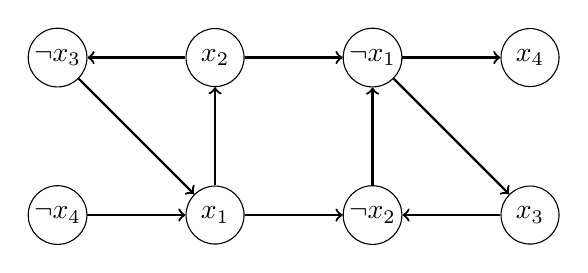
\begin{tikzpicture}[scale=1.0,minimum size=2pt]
\node[draw, circle, inner sep=1.3pt] (1) at (1,2) {$\lnot x_3$};
\node[draw, circle] (2) at (3,2) {$x_2$};
\node[draw, circle, inner sep=1.3pt] (3) at (1,0) {$\lnot x_4$};
\node[draw, circle] (4) at (3,0) {$x_1$};
\node[draw, circle, inner sep=1.3pt] (5) at (5,2) {$\lnot x_1$};
\node[draw, circle] (6) at (7,2) {$x_4$};
\node[draw, circle, inner sep=1.3pt] (7) at (5,0) {$\lnot x_2$};
\node[draw, circle] (8) at (7,0) {$x_3$};
 
\path[draw,thick,->] (1) -- (4);
\path[draw,thick,->] (4) -- (2);
\path[draw,thick,->] (2) -- (1);
\path[draw,thick,->] (3) -- (4);
\path[draw,thick,->] (2) -- (5);
\path[draw,thick,->] (4) -- (7);
\path[draw,thick,->] (5) -- (6);
\path[draw,thick,->] (5) -- (8);
\path[draw,thick,->] (8) -- (7);
\path[draw,thick,->] (7) -- (5);
\end{tikzpicture}
\end{center}

Lausekkeen $L_2$ verkosta taas tulee:
\\
\begin{center}
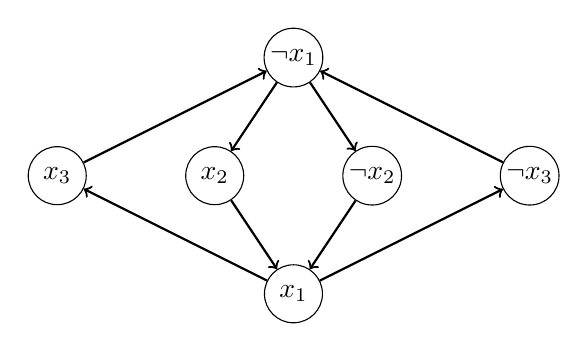
\begin{tikzpicture}[scale=1.0,minimum size=2pt]
\node[draw, circle] (1) at (1,2) {$x_3$};
\node[draw, circle] (2) at (3,2) {$x_2$};
\node[draw, circle, inner sep=1.3pt] (3) at (5,2) {$\lnot x_2$};
\node[draw, circle, inner sep=1.3pt] (4) at (7,2) {$\lnot x_3$};
\node[draw, circle, inner sep=1.3pt] (5) at (4,3.5) {$\lnot x_1$};
\node[draw, circle] (6) at (4,0.5) {$x_1$};

\path[draw,thick,->] (1) -- (5);
\path[draw,thick,->] (4) -- (5);
\path[draw,thick,->] (6) -- (1);
\path[draw,thick,->] (6) -- (4);
\path[draw,thick,->] (5) -- (2);
\path[draw,thick,->] (5) -- (3);
\path[draw,thick,->] (2) -- (6);
\path[draw,thick,->] (3) -- (6);
\end{tikzpicture}
\end{center}

Verkon rakenne kertoo, onko 2SAT-ongelmalla ratkaisua.
Jos on jokin muuttuja $x_i$ niin,
että $x_i$ ja $\lnot x_i$ ovat samassa
vahvasti yhtenäisessä komponentissa,
niin ratkaisua ei ole olemassa.
Tällöin verkossa on polku sekä $x_i$:stä
$\lnot x_i$:ään että $\lnot x_i$:stä $x_i$:ään,
eli kumman tahansa arvon valitseminen
muuttujalle $x_i$ pakottaisi myös valitsemaan
vastakkaisen arvon, mikä on ristiriita.

Lausekkeen $L_1$ verkossa tällaista
muuttujaa $x_i$ ei ole,
mikä tarkoittaa, että ratkaisu on olemassa.
Lausekkeen $L_2$ verkossa taas kaikki solmut
kuuluvat samaan vahvasti yhtenäiseen komponenttiin,
eli ratkaisua ei ole olemassa.

Jos ratkaisu on olemassa, muuttujien arvot saa selville
käymällä komponenttiverkko läpi käänteisessä
topologisessa järjestyksessä.
Tällöin verkosta otetaan käsittelyyn ja poistetaan
joka vaiheessa komponentti,
josta ei lähde kaaria muihin jäljellä
oleviin komponentteihin.

Jos komponentin muuttujille ei ole vielä valittu arvoja,
ne saavat komponentin mukaiset arvot.
Jos taas arvot on jo valittu, niitä ei muuteta.
Näin jatketaan, kunnes jokainen muuttuja on saanut arvon.

Lausekkeen $L_1$ verkon komponenttiverkko on seuraava:
\\
\begin{center}
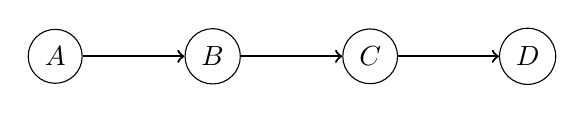
\begin{tikzpicture}[scale=1.0]
\node[draw, circle] (1) at (0,0) {$A$};
\node[draw, circle] (2) at (2,0) {$B$};
\node[draw, circle] (3) at (4,0) {$C$};
\node[draw, circle] (4) at (6,0) {$D$};

\path[draw,thick,->] (1) -- (2);
\path[draw,thick,->] (2) -- (3);
\path[draw,thick,->] (3) -- (4);
\end{tikzpicture}
\end{center}

Komponentit ovat
$A = \{\lnot x_4\}$,
$B = \{x_1, x_2, \lnot x_3\}$,
$C = \{\lnot x_1, \lnot x_2, x_3\}$ sekä
$D = \{x_4\}$.
Ratkaisun muodostuksessa
käsitellään ensin komponentti $D$,
josta $x_4$ saa arvon tosi.
Sitten käsitellään komponentti $C$,
josta $x_1$ ja $x_2$ tulevat epätodeksi
ja $x_3$ tulee todeksi.
Kaikki muuttujat ovat saaneet arvon,
joten myöhemmin käsiteltävät
komponentit $B$ ja $A$ eivät vaikuta enää ratkaisuun.

Huomaa, että tämän menetelmän toiminta
perustuu verkon erityiseen rakenteeseen.
Jos solmusta $x_i$ pääsee
solmuun $x_j$,
josta pääsee solmuun $\lnot x_j$,
niin $x_i$ ei saa koskaan arvoa tosi.
Tämä johtuu siitä, että
solmusta $\lnot x_j$ täytyy
päästä myös solmuun $\lnot x_i$,
koska kaikki riippuvuudet
ovat verkossa molempiin suuntiin.
Niinpä sekä $x_i$ että $x_j$
saavat varmasti arvokseen epätosi.

\index{3SAT-ongelma}

2SAT-ongelman vaikeampi versio on \key{3SAT-ongelma},
jossa jokainen lausekkeen osa on muotoa
$(a_i \lor b_i \lor c_i)$.
Tämän ongelman ratkaisemiseen \textit{ei}
tunneta tehokasta menetelmää,
vaan kyseessä on NP-vaikea ongelma.


